\documentclass[aspectratio=169, 10pt]{beamer}
\title{\textbf{Exchange rate and Production network}}
\subtitle{Brown bag seminar}
\author{Sugarkhuu Radnaa}
\institute[]{Bonn Graduate School of Economics}
\date{June, 2026}
\usetheme{default}
\usepackage[T1]{fontenc}
\usepackage{lmodern}
\usepackage{amssymb}
\usepackage{amsmath}
\usepackage{xcolor}
\usepackage{booktabs}
\usepackage{natbib}
\usepackage{mathtools}
\usepackage{bm}
\usepackage{tikz}
\usepackage{pgfplots}
\pgfplotsset{compat=1.18}
\usetikzlibrary{arrows.meta, positioning}

\setbeamercolor{normal text}{fg=black}
\setbeamercolor{title}{fg=black}
\setbeamercolor{subtitle}{fg=black}
\setbeamercolor{itemize item}{fg=customgreen}
\setbeamertemplate{frametitle}[default][left]
\setbeamertemplate{items}[circle]
\definecolor{customgreen}{RGB}{10, 43, 19}
\setbeamercolor{frametitle}{bg=customgreen, fg=white}
\setlength{\headheight}{1.25cm}

\setbeamertemplate{footline}{%
  \hspace*{1em}\scriptsize\insertframenumber{} / \inserttotalframenumber%
  \hfill%
}

\newcommand{\bpi}{\bm{\pi}}
\newcommand{\ty}{\tilde{y}}
\newcommand{\tA}{\tilde{A}}
\newcommand{\bom}{\bm{\omega}_F}

\pgfplotsset{
  slide fig/.style={
    tick label style={font=\tiny},
    label style={font=\tiny},
    title style={font=\tiny, align=center},
    legend style={font=\tiny, draw=none, fill=none},
    grid=both, grid style={dotted, gray!35},
    axis line style={gray!60},
    every axis plot/.append style={line width=1pt},
  }
}

\begin{document}

%--------------------------------------------------------------
\begin{frame}
  \titlepage
  \begin{center}
    \small Building on: Rubbo (2024) \emph{Networks, Phillips Curves, and Monetary Policy}
  \end{center}
\end{frame}

%==============================================================
\begin{frame}{Rubbo (2024): Key Results}
%==============================================================

\begin{columns}[t]
\column{0.56\textwidth}

{\footnotesize \textbf{Full model system} ($N$ sectors, Calvo $\hat\delta_i$, IO network $\Omega$):}
\vspace{-3pt}
{\scriptsize\begin{align*}
\text{IS:} &\quad \ty_t = \mathbb{E}\ty_{t+1} - \tfrac{1}{\gamma}(i_t - \mathbb{E}\pi^C_{t+1} - r^{nat}_t) \\[1pt]
\text{MC:} &\quad \bm{mc}_t = \bm{\alpha}w_t + \Omega\bm{p}_t - \log\mathbf{A}_t \\[1pt]
\text{NKPC:} &\quad \bpi_t = \rho(I{-}\mathcal{V})\mathbb{E}\bpi_{t+1} + \mathcal{B}(\gamma{+}\varphi)\ty_t - \mathcal{V}\bm{\chi}_t \\[1pt]
\text{CPI:} &\quad \pi^C_t = \bm{\beta}^T\bpi_t \\[1pt]
\text{Policy:} &\quad i_t = r^{nat}_t + \phi_\pi\pi^C_t + \phi_y\ty_t
\end{align*}}
\vspace{-5pt}
{\scriptsize $\mathcal{B}{=}\tfrac{(\gamma+\varphi)\Delta(I-\Omega\Delta)^{-1}\bm{\alpha}}{\kappa}$;\; $\bm{\chi}_t \equiv \log\mathbf{A}_t$ (TFP);\; $\mathcal{V}{=}\Delta(I{-}\Omega\Delta)^{-1}$}

\vspace{3pt}
{\footnotesize \textbf{Divine Coincidence (Prop.\ 1):} unique index with \emph{no} cost-push:}
\vspace{-4pt}
\[\footnotesize \pi^{DC}_t = \rho\,\mathbb{E}\pi^{DC}_{t+1} + \tfrac{\gamma+\varphi}{\Lambda^{DC}}\ty_t,\quad w^{DC}_i \propto \lambda_i\tfrac{1-\hat\delta_i}{\hat\delta_i}\]
\vspace{-6pt}
{\footnotesize \textbf{Unique:} $\mathcal{V}$ rank $N{-}1$ $\Rightarrow$ one-dim.\ null space. Optimal policy = target $\pi^{DC}_t$.}

\vspace{2pt}
{\footnotesize \textbf{Welfare (Prop.\ 3):} $\mathbb{W} = \tfrac{1}{2}\sum_t\rho^t[(i)\;\ty_t^2 + (ii)\;\text{within-sector} + (iii)\;\text{cross-sector}]$.

DC targeting minimizes all three terms simultaneously.}

\column{0.40\textwidth}

\vspace{-4pt}
\begin{center}
{\tiny \textbf{Welfare loss by policy rule (illustrative)}}\\[3pt]
\begin{tikzpicture}
\begin{axis}[
  slide fig,
  xbar, width=5.0cm, height=3.4cm,
  bar width=9pt,
  xlabel={\tiny Welfare loss (rel.\ units)},
  symbolic y coords={DC index, Output gap, CPI},
  ytick=data,
  yticklabel style={font=\tiny},
  xmin=0, xmax=82,
  xmajorgrids=true, ymajorgrids=false,
  nodes near coords,
  nodes near coords style={font=\tiny, xshift=2pt},
  every axis plot/.append style={fill=customgreen!45!white, draw=customgreen!70!black},
]
\addplot coordinates {(8,DC index) (36,Output gap) (64,CPI)};
\end{axis}
\end{tikzpicture}
\end{center}

\vspace{-4pt}
{\tiny \textit{DC targeting achieves the lowest welfare loss by eliminating cost-push distortion. Rubbo (2024) quantifies using US BEA IO data.}}

\end{columns}
\end{frame}

%==============================================================
\begin{frame}{SOE Model: Structural Equations}
%==============================================================

\begin{columns}[t]
\column{0.50\textwidth}

{\footnotesize \textbf{Household} ($\gamma$: risk aversion, $\varphi$: inv.\ labor elasticity)}
\vspace{-3pt}
{\scriptsize\begin{align*}
\max\; & \mathbb{E}_0\!\sum_t \beta^t\!\left[\tfrac{C_t^{1-\gamma}}{1-\gamma} - \tfrac{L_t^{1+\varphi}}{1+\varphi}\right] \\[0pt]
\text{s.t.}\; & P^C_t C_t + B_t + E_t B^*_t = (1{+}i_{t-1})B_{t-1} \\[-2pt]
              & \hspace{2.5cm}+\, E_t(1{+}i^*)B^*_{t-1} + W_t L_t + \Pi_t \\[0pt]
\text{FOC $B$:}\; & \lambda_t = \beta(1{+}i_t)\,\mathbb{E}_t[\lambda_{t+1}/\pi^C_{t+1}] \\[0pt]
\text{FOC $B^*$:}\; & \lambda_t = \beta(1{+}i^*_t)\,\mathbb{E}_t[\lambda_{t+1}(E_{t+1}/E_t)/\pi^C_{t+1}] \\[0pt]
\text{Labor:}\; & W_t/P^C_t = C_t^{\gamma} L_t^{\varphi}
\end{align*}}
\vspace{-5pt}
{\scriptsize $\lambda_t{\equiv}C_t^{-\gamma}$;\; $\pi^C_{t+1}{\equiv}P^C_{t+1}/P^C_t$;\; FOC\,$B^*\div$FOC\,$B$ $\Rightarrow$ UIP below}

\vspace{3pt}
{\footnotesize \textbf{International block} ($E_t$: nominal ER, $P^*_t$: foreign price)}
\vspace{-3pt}
{\scriptsize\begin{align*}
\text{LOP:}\; & P_{Ft} = E_t P^*_t \\[0pt]
\text{CPI:}\; & P^C_t = \textstyle\prod_i P_{it}^{\beta_i}\cdot (E_t P^*_t)^{\alpha_F} \\[0pt]
\text{ToT:}\; & \tau_t = E_t P^*_t / P^H_t \\[0pt]
\text{UIP:}\; & (1{+}i_t) = (1{+}i^*_t)\,\mathbb{E}_t[E_{t+1}/E_t]\cdot(1{+}\psi_t)/(1{+}\nu_t)
\end{align*}}

\column{0.46\textwidth}

{\footnotesize \textbf{Firm $i$: Cobb-Douglas production, Calvo pricing}}
\vspace{-3pt}
{\scriptsize\begin{align*}
\text{Prod.:}\; & Y_{it} = A_{it}\, L_{it}^{\alpha_i}\prod_j M_{ijt}^{\omega_{ij}} M_{Fit}^{\omega_{Fi}} \\[0pt]
\text{MC:}\; & MC_{it} = \frac{W_t^{\alpha_i}\prod_j P_{jt}^{\omega_{ij}}(E_t P^*_t)^{\omega_{Fi}}}{A_{it}} \\[0pt]
\text{Calvo:}\; & \begin{cases} \text{prob } (1{-}\hat\delta_i): \text{ reset } \tilde{P}_{it} = \tfrac{\varepsilon}{\varepsilon-1}\mathbb{E}_t[\text{PV of MC}] \\ \text{prob } \hat\delta_i: \text{ keep } P_{i,t-1} \end{cases} \\[1pt]
\text{Price:}\; & P_{it}^{1-\varepsilon} = (1{-}\hat\delta_i)\tilde{P}_{it}^{1-\varepsilon} + \hat\delta_i P_{i,t-1}^{1-\varepsilon}
\end{align*}}

\vspace{1pt}
{\footnotesize \textbf{Market clearing}}
\vspace{-3pt}
{\scriptsize\begin{align*}
\text{Goods:}\; & Y_{it} = C_{Hit} + X_{it} + \textstyle\sum_j M_{jit} \\[0pt]
\text{Labor:}\; & L_t = \textstyle\sum_i N_{it}
\end{align*}}
\vspace{-4pt}
{\scriptsize $\Rightarrow$ Log-linearize $+$ take gaps around flex-price equilibrium $\Rightarrow$ IS, MC, NKPC (next slide).}

\end{columns}
\end{frame}

%==============================================================
\begin{frame}{Small Open Economy Extension}
%==============================================================

{\footnotesize \textbf{What I add:} Import sector $+$ UIP $+$ law of one price. Exchange rate $e_t$ enters marginal cost.}

\vspace{1pt}
\begin{columns}[t]
\column{0.52\textwidth}

{\footnotesize \textbf{Full system} (\textcolor{customgreen}{\textbf{green}} = new SOE terms):}
\vspace{-4pt}
{\scriptsize\begin{align*}
\text{IS:} &\quad \ty_t = \mathbb{E}\ty_{t+1} - \tfrac{1}{\gamma}(i_t - \mathbb{E}\pi^C_{t+1} - r^{nat}_t) \textcolor{customgreen}{+\,\Delta\tau_t} \\[0pt]
\text{MC:} &\quad \bm{mc}_t = \bm{\alpha}w_t + \Omega\bm{p}_t \textcolor{customgreen}{+ \bom(p^*_t{+}e_t)} - \log\mathbf{A}_t \\[0pt]
\text{NKPC:} &\quad \bpi_t = \rho(I{-}\mathcal{V})\mathbb{E}\bpi_{t+1} + \mathcal{B}(\gamma{+}\varphi)\ty_t - \mathcal{V}\bm{\chi}_t \textcolor{customgreen}{+ \Gamma\Delta e_t} \\[0pt]
\text{UIP:} &\quad \textcolor{customgreen}{i_t - i^* = \mathbb{E}\Delta e_{t+1} + \psi_t - \nu_t} \\[0pt]
\text{Policy:} &\quad i_t = r^{nat}_t + \phi_\pi\pi^C_t + \phi_y\ty_t;\;\textcolor{customgreen}{\nu_t^*:\;\text{FX intervention}}
\end{align*}}
\vspace{-7pt}
{\scriptsize $p^*_t$: foreign price;\; $i^*$: foreign rate;\; $e_t$: log ER;\; $\nu_t$: FXint

\vspace{5pt}

$\Gamma{=}\tA\bom/\kappa$,\; $\tA{=}\Delta(I{-}\Omega\Delta)^{-1}$,\; $\bom$: import intensity shares}

\vspace{0pt}
{\footnotesize \textbf{Changes from Rubbo:}
\begin{enumerate}\setlength{\itemsep}{0pt}\setlength{\topsep}{1pt}
  \item IS: terms-of-trade effect $\Delta\tau = p^*{+}e - p^H$
  \item MC: imported input costs enter price-setting
  \item NKPC: ER cost-push $\Gamma\Delta e_t$ (network amplified)
  \item UIP $+$ $\nu_t$: ER dynamics close the model
\end{enumerate}
\textbf{Two cost-push channels} (TFP $+$ ER) $\Rightarrow$ DC breaks down}

\column{0.44\textwidth}

\vspace{-2pt}
\begin{center}
{\tiny \textbf{Production network with import sector}}\\[4pt]
\begin{tikzpicture}[scale=0.65,
  sector/.style={circle, draw=customgreen!80!black, fill=customgreen!12, thick,
                 minimum size=1.1cm, font=\tiny, align=center},
  foreign/.style={rectangle, draw=gray!60, dashed, thick, fill=gray!10,
                  font=\tiny, align=center, minimum width=1.3cm, minimum height=0.6cm},
  ioarr/.style={-{Stealth[scale=0.9]}, thick, customgreen!70!black},
  farr/.style={-{Stealth[scale=0.9]}, dashed, gray!65, thick},
]
\node[sector] (S1) at (0.0, 2.4) {Sector 1\\(Energy)};
\node[sector] (S2) at (2.4, 2.4) {Sector 2\\(Mfg)};
\node[sector] (S3) at (1.2, 0.8) {Sector 3\\(Serv.)};
\node[foreign] (F)  at (4.0, 1.6) {$e_t{+}p^*$\\Import};
\draw[ioarr] (S1) to[bend left=18]  node[above, font=\tiny] {$\omega_{21}$} (S2);
\draw[ioarr] (S2) to[bend left=10]  node[right, font=\tiny] {$\omega_{32}$} (S3);
\draw[ioarr] (S1) to[bend right=10] node[left,  font=\tiny] {$\omega_{31}$} (S3);
\draw[ioarr] (S3) to[bend left=15] (S1);
\draw[farr]  (F)  to[bend left=15]  node[right, font=\tiny, yshift=2pt] {$\omega_{F2}$} (S2);
\draw[farr]  (F)  to[bend right=5]  node[below right, font=\tiny] {$\omega_{F3}$} (S3);
\draw[farr]  (F)  to[bend right=28] node[above, font=\tiny] {$\omega_{F1}$} (S1);
\end{tikzpicture}
\end{center}

\vspace{-2pt}
{\tiny \textit{Dashed: new SOE import flows. Depreciation ($\Delta e_t{>}0$) raises imported input costs and propagates through the IO network via $\Gamma$.}}

\end{columns}
\end{frame}

%==============================================================
\begin{frame}{Network Amplification: Upstream, Downstream, Centrality}
%==============================================================

\begin{columns}[t]
\column{0.50\textwidth}

{\footnotesize \textbf{Leontief expansion of ER pass-through $\Gamma_i$:}}
\vspace{-4pt}
{\scriptsize\begin{align*}
\Gamma_i = \frac{\hat\delta_i}{\kappa}\Big[
  \underbrace{\omega_{Fi}}_{\text{direct}} +
  \underbrace{\textstyle\sum_j \omega_{ij}\hat\delta_j\omega_{Fj}}_{\text{suppliers}} +
  \underbrace{\textstyle\sum_{j,k} \omega_{ij}\hat\delta_j\omega_{jk}\hat\delta_k\omega_{Fk}}_{\text{2nd order}} + \cdots\Big]
\end{align*}}
\vspace{0pt}
{\footnotesize Each round discounted by rigidities $\hat\delta$ along the chain.\\[5pt]


\textbf{Upstream $u$:} high $\omega_{Fu}$ $\Rightarrow$ raises $\Gamma_i$ for all customers; stickier upstream absorbs into markup, lower pass-through.\\[2pt]
\textbf{Downstream $d$:} high $\Gamma_d$ even if own $\omega_{Fd}$ low.\\[2pt]
\textbf{DC breakdown:} requires $\bom \propto (I{-}\Omega\Delta)\bm{\phi}^{DC}$ --- fails empirically.\\[2pt]
\textbf{Welfare:} $\bm{\lambda}^T\Gamma = \sum_i\lambda_i\Gamma_i$ --- Domar $\times$ $\Gamma_i$ drives macro cost.}

\column{0.47\textwidth}

\vspace{-4pt}
\begin{center}
{\tiny \textbf{Centrality $\lambda_i$ vs ER sensitivity $\Gamma_i$ (illustrative)}}\\[2pt]
\begin{tikzpicture}
\begin{axis}[
  slide fig,
  width=5.4cm, height=4.3cm,
  xlabel={\tiny Domar weight $\lambda_i$},
  ylabel={\tiny ER pass-through $\Gamma_i$},
  xmin=0.03, xmax=0.23,
  ymin=0.00, ymax=0.22,
  xtick={0.05,0.10,0.15,0.20},
  ytick={0.00,0.05,0.10,0.15,0.20},
]
\addplot[only marks, mark=*, mark size=2.2pt,
         mark options={fill=customgreen!60, draw=customgreen!80!black}]
  coordinates {
    (0.19, 0.17)
    (0.07, 0.15)
    (0.10, 0.13)
    (0.12, 0.18)
    (0.09, 0.02)
    (0.14, 0.04)
    (0.06, 0.07)
    (0.08, 0.05)
  };
\node[font=\tiny, anchor=west]  at (axis cs:0.195, 0.170) {Mfg};
\node[font=\tiny, anchor=east]  at (axis cs:0.065, 0.150) {Energy};
\node[font=\tiny, anchor=north] at (axis cs:0.100, 0.120) {Chem};
\node[font=\tiny, anchor=south] at (axis cs:0.120, 0.185) {Mach};
\node[font=\tiny, anchor=north] at (axis cs:0.090, 0.015) {Finance};
\node[font=\tiny, anchor=north] at (axis cs:0.140, 0.030) {Services};
\node[font=\tiny, anchor=east]  at (axis cs:0.055, 0.070) {Transp};
\node[font=\tiny, anchor=north] at (axis cs:0.080, 0.043) {Retail};
\node[font=\tiny, text=gray!70, align=center] at (axis cs:0.195, 0.205)
  {high\\risk};
\draw[dashed, gray!50, thin] (axis cs:0.13, 0.00) -- (axis cs:0.13, 0.22);
\draw[dashed, gray!50, thin] (axis cs:0.03, 0.10) -- (axis cs:0.23, 0.10);
\end{axis}
\end{tikzpicture}
\end{center}
{\tiny \textit{Upper-right: high centrality $+$ high import intensity --- sectors where ER shocks generate the largest welfare costs.}}
\end{columns}

\end{frame}

%==============================================================
\begin{frame}{Core Result: DC Breakdown and Managed Float}
%==============================================================

\begin{columns}[t]
\column{0.48\textwidth}

{\footnotesize \textbf{DC breaks down under float (Prop.\ 1$'$):}

Cost-push-free index requires two conditions:}
\vspace{-5pt}
\[\small \underbrace{\bm{\phi}^T\mathcal{V} = \mathbf{0}^T}_{\text{pins }\bm{\phi}=\bm{\phi}^{DC}} \quad \text{AND} \quad \underbrace{\bm{\phi}^T\Gamma = 0}_{\text{generically fails}}\]
\vspace{1pt}
{\footnotesize Two conditions, one unknown $\bm{\phi}$ $\Rightarrow$ no solution.}

\vspace{3pt}
{\footnotesize
\begin{tabular}{@{}lccc@{}}
\toprule
 & \textbf{Float} & \textbf{Peg} & \textbf{Managed} \\
\midrule
ER cost-push & Free & Zero & $\perp\bm{\phi}^{DC}$ \\
MP independence & Full & None & Full \\
DC survives? & No & Yes & Restored \\
Optimal & None & DC & DC $+$ $\nu_t^*$ \\
\bottomrule
\end{tabular}
}

\vspace{4pt}
{\footnotesize \textbf{Managed float:} $\;i_t{-}i^* = \mathbb{E}\Delta e_{t+1} {+} \psi_t {-} \nu_t$

Optimal $\nu_t^*$: $(\bm{\phi}^{DC})^T\Gamma\,\Delta e_t(\nu_t^*) {=} 0$.
Restores: $\pi_t^{DC} {=} \rho\mathbb{E}\pi_{t+1}^{DC} {+} \tfrac{\gamma+\varphi}{\Lambda^{DC}}\ty_t$. Two instruments, two targets.}

\column{0.49\textwidth}

\vspace{-4pt}
\begin{center}
{\tiny \textbf{IRF: CPI inflation response to 1\% ER depreciation (illustrative)}}\\[2pt]
\begin{tikzpicture}
\begin{axis}[
  slide fig,
  width=6.0cm, height=3.0cm,
  xlabel={\tiny Quarters},
  ylabel={\tiny CPI inflation (\%)},
  xmin=0.5, xmax=10.5,
  ymin=-0.02, ymax=0.55,
  xtick={1,2,...,10},
  ytick={0,0.1,0.2,0.3,0.4,0.5},
  legend style={font=\tiny, at={(0.97,0.97)}, anchor=north east,
                row sep=-3pt, inner sep=2pt},
]
\addplot[thick, customgreen!85!black]
  coordinates {(1,0.45)(2,0.33)(3,0.24)(4,0.18)(5,0.13)(6,0.10)(7,0.07)(8,0.05)(9,0.04)(10,0.03)};
\addlegendentry{Float}
\addplot[thick, gray!60!black, dashed]
  coordinates {(1,0.18)(2,0.09)(3,0.04)(4,0.02)(5,0.01)(6,0.00)(7,0.00)(8,0.00)(9,0.00)(10,0.00)};
\addlegendentry{Managed float}
\addplot[thick, gray!40, dotted]
  coordinates {(1,0.00)(2,0.00)(3,0.00)(4,0.00)(5,0.00)(6,0.00)(7,0.00)(8,0.00)(9,0.00)(10,0.00)};
\addlegendentry{Peg}
\end{axis}
\end{tikzpicture}

\vspace{1pt}
{\tiny \textbf{Welfare loss by FX regime (illustrative)}}\\[1pt]
\begin{tikzpicture}
\begin{axis}[
  slide fig,
  xbar, width=5.8cm, height=3.0cm,
  bar width=7pt,
  xlabel={\tiny Welfare loss (rel.\ units)},
  symbolic y coords={Managed, Peg, Float},
  ytick=data,
  yticklabel style={font=\tiny},
  xmin=0, xmax=115,
  xmajorgrids=true, ymajorgrids=false,
  nodes near coords,
  nodes near coords style={font=\tiny},
  every axis plot/.append style={fill=customgreen!40!white, draw=customgreen!70!black},
]
\addplot coordinates {(28,Managed) (52,Peg) (100,Float)};
\end{axis}
\end{tikzpicture}
\end{center}

\end{columns}

\end{frame}

%==============================================================
\begin{frame}{Four Quantitative Experiments}
%==============================================================

{\footnotesize \textbf{1. IRF to ER shock} --- Simulate a 1\% depreciation. Track sector-level CPI responses; plot $\lambda_i$ vs $\Gamma_i$ to identify which sectors drive aggregate inflation via the IO network.}

\vspace{4pt}
{\footnotesize \textbf{2. Welfare: float vs peg vs managed float} --- Compare $\mathbb{W} = \tfrac{1}{2}\sum_t\rho^t[\ty_t^2 + \text{dispersion} + \text{misalloc.}]$ across three FX regimes for identical shocks. Quantifies the cost of DC breakdown under float and the gain from $\nu_t$.}

\vspace{4pt}
{\footnotesize \textbf{3. DC breakdown test} --- Measure the two cost-push channels:
\[\scriptsize \underbrace{\mathcal{V}\bm{\chi}_t}_{\text{TFP channel}} \quad \text{vs} \quad \underbrace{\Gamma\Delta e_t}_{\text{ER channel}}\]
\vspace{-6pt}
If comparable in magnitude but not collinear, no single index eliminates both. Quantifies \emph{how much} DC breaks down in calibrated data.}

\vspace{4pt}
{\footnotesize \textbf{4. Optimal FX intervention $\nu_t^*$} --- Solve for $\nu_t^*$ satisfying $(\bm{\phi}^{DC})^T\Gamma\,\Delta e_t(\nu_t^*) = 0$, restoring the DC index under float. Two instruments $(i_t,\nu_t)$, two targets (output gap, DC index).}
\end{frame}

%==============================================================
\begin{frame}{Simulation Design and Roadmap}
%==============================================================

\begin{columns}[t]
\column{0.52\textwidth}

{\footnotesize \textbf{Code: extends Rubbo's Matlab directly}}

\vspace{3pt}
{\scriptsize
\begin{tabular}{@{}p{2.9cm}p{4.0cm}@{}}
\toprule
\textbf{Module} & \textbf{Task} \\
\midrule
\texttt{parameters\_soe.m} & Load import shares $\bom$; compute $\Gamma$ \\
\texttt{pol\_fct\_soe.m} & Augment state with $e_t$, UIP \\
\texttt{IRFs\_soe.m} & IRFs to ER \& MP shocks \\
\texttt{simul\_soe.m} & Monte Carlo: 3 FX regimes \\
\texttt{welfare\_soe.m} & Add ER misallocation term \\
\bottomrule
\end{tabular}
}

\vspace{3pt}
{\footnotesize \textbf{Augmented state space:}}
\vspace{-6pt}
{\small\[T_{\text{SOE}} = \begin{pmatrix} T_{\text{Rubbo}} & \Gamma \\ \bm{0} & \rho_e \end{pmatrix},\quad e_t = \rho_e e_{t-1} + \varepsilon_t^e\]}
\vspace{-6pt}

\column{0.44\textwidth}

{\footnotesize \textbf{Theory so far:}}

\vspace{2pt}
{\footnotesize
\begin{tabular}{@{}ll@{}}
$\checkmark$ & Rubbo lemmas/props verified \\
$\checkmark$ & SOE Phillips curve ($+\Gamma\Delta e_t$) \\
$\checkmark$ & DC breakdown (two conditions) \\
$\checkmark$ & Upstream/downstream decomp. \\
$\checkmark$ & Managed float ($\nu_t^*$) \\
$\checkmark$ & Welfare SOE extension \\
\end{tabular}
}

\vspace{4pt}
{\footnotesize \textbf{Remaining (July 22):}

\begin{tabular}{@{}ll@{}}
$\square$ & IO data: sector import shares $\bom$ \\
$\square$ & Implement \texttt{parameters\_soe.m} \\
$\square$ & Augmented state space \\
$\square$ & Welfare plots \\
$\square$ & Experiments \\
% $\square$ & Paper sections 2--4 \\
\end{tabular}
}

\vspace{4pt}
{\scriptsize
\begin{tabular}{@{}lll@{}}
\toprule
 & \textbf{Rubbo} & \textbf{This paper} \\
\midrule
Economy & Closed & SOE + ER \\
Cost-push & 1 channel & 2 channels \\
DC index & Unique & Breaks down \\
Optimal MP & DC target & DC + $\nu_t^*$ \\
\bottomrule
\end{tabular}
}

\end{columns}

\end{frame}

\end{document}
